\chapter{Related Works}

\section{Citizen science}

The challenge of designing scientific discovery games is that interaction design must be optimized for suitable human interactions in the exploration process while still respecting the scientific requirements \cite{cooper2010challenge}. Fold-it is able to design new drugs by leveraging the creative side of humans brains to organize proteins. The game originally attracted the biochemist community, but the creator, explains during Science Friday on Public Radio International, ``most biochemists quickly left the game because they were pummeled by ordinary people who had incredible spatial recognition skills." \cite{sciencefriday2014}

\subsection{Fold-it}

Fold-it coins the term scientific discovery games \cite{cooper2010challenge} to describe their system. Scientific discovery games are differentiated from general citizen science games because they focus on the problem solving ability of humans to solve computationaly difficult problems \cite{cooper2010challenge}. Fold-it incorporates many traditional aspects of game design; the highlight of Fold-it's design are the use of introductory levels to draw newcomers and explain the mechanics and the requirement that the game still be fun. 

Complex graphical structures are scientifically necessary to illustrate protein structures, but they must also promote human ability to understand those complex structures \cite{cooper2010challenge}. The visualizations in scientific discovery games have several requirements: they must ``reflect and illuminate the natural rules of the system" \cite{cooper2010challenge}, ``manage and hide the complexity of the system" \cite{cooper2010challenge}, and be ``approachable by players" \cite{cooper2010challenge} who have no knowledge of the scientific problem. They should be inviting and fun, not reminiscent of high school science textbooks. In order to make the game approachable, the protein has a bright, cartoonish feel. 

The visualizations of the game are mostly cohesive, but it obvious that the aesthetics were not the priority when optimizing the players first interactions with the game. For instance the login page has an empty box which doesn't seem to contain any information, but still blocks a significant portion of my vision. There are some icons indicating my options, but they aren't necessarily carefuly chosen. The ``Play Offline" icon (two computers with a do-not-enter sybmol) differs significantly from the ``Play Online" button which is a smiley face.

The interactions within the puzzle are intutive and simplified. The creators of Fold-it emphasized interactions that are sufficient to explore, yet intuitive and fun \cite{cooper2010challenge}. Fold-it prototyped games that used sliders to indirectly manipulate the protein, but users found them unintuitive \cite{cooper2010challenge}. Fold-it highlights ``touchability"--the feeling of grabbing and manipulating protein structures with my mouse, as opposed to rearranging sliders for the same effect \cite{cooper2010challenge}. Clicking and dragging with the mouse produces real-time feedback and enables the corrective cycle. While rearrange the shape of the major backbone, there are large pulsing red shapes that indicate when the structure creates physically impossible ``clashes" or ``voids" which warrants correction.

While the sound effects associated with Fold-it aren't particularly pleasing or reminiscent of proteins or this metaphore, they are indicitive of my current state. Sounds accompany different states including dragging and pulling certain elements or using one of the predetermined procedural ``shake" or ``wiggle" functions. After completing a tutorial step, a simple ``Congratulations!" message flashes quickly. The primary motivator to complete certain shapes depends entirely on watching the score increase and decrease the shape of the protein is modified. This is intentional to ``direct players towards the solution" \cite{cooper2010challenge} and is the only significant indicator whether some seemingly-trivial motions of the protein are good or bad for its overall structure.

Fold-it's tutorial are designed to teach non-experts by introducing concepts one level at a time. It is helpful for those who want to just jump right into the puzzles and start folding proteins. The first thing you can do in Fold-it is play with the structure of a protein and begin folding. The higher-level concepts are omitted. There are text bubbles that pop up and guide your mouse to the right tools and options.

Fold it also includes more traditional game elements to keep serious players solving puzzles. The leaderboards are noted by Cooper to be highly compettive \cite{cooper2010challenge}.

\subsection{The Milky Way Project}

The Spitzer Space Telescope gathers infrared light from deep within the Milky Way \cite{milkyway2014}. Scientists have been collecting data for the last 20 years trying to understand how certain diffuse materials collect and create recurring structures and patterns. Users are shown bit-sized images of the Milky Way and provided tools to identify galaxies, star cluters, and egos. Image recognition is a common citizen science task because computationally identifying images is still a field of constant research. Fortunately, humans are surprisingly good with our eyes to make identifying irregular objects easy, but unfortunately not every person can identify each image precisely. The Milky Way project gives the same image to many people and compares the results to settle on a ``correct" identification. Scientists at the University of Oxford leverage the patterns identified by ``untrained" citizens to train their machine learning algorithm, Brut, which is then trained to discover ``bubbles" in the Milky Way \cite{milkyway2014}.

The interface itself is very simple and it is built for a simple task--identifying certain shapes in images. The simplicity of The Milky Way Project should not be overlooked; they have narrowed down the problem scope to an easily digestible size which makes recognition quick. The tutorial system allows users to practice on an image or automatically simulates mouse clicks that complete the tutorial for them. It is simply, but short and effective because it imitates exacty what the player will be doing in the game. There is no description of what a star cluster or a bubble represents without navigating to the ``Science" page. The primary motivation to complete these tasks is simply to partake in science, though images of stars are not displeasing.

\subsection{Cure to Play: Genes in Space}

Genes in Space is interesting because it applies a much more traditional game atmosphere designed around abstrating out the core scientific element. The game is based on the fundamental structure of DNA chromosomes. Cancer cells exhibit certain genetic faults--changes in A, C, G, or T--that result in huge changes in parts of chromosomes known as copy number alterations. (Can the power of the public help personalise cancer treatment?) Copy number alterations can help predict the course of the disease, but it is difficult for computers to identify copy number changes. The human eye is great at detecting these shifts.

Software to identify these differences in DNA micro arrays exists, but it is unable to identify as many patterns as humans can \cite{canthepower}. Software has proven to take significantly identify this problem, but without results published from Genes in Space, it is impossible to compare the two methods \cite{curtis2012genomic}.

Developers from Google, Amazon, and Facebook created the game during a weekend known as GameJam during March 2013 \cite{canthepower}. The DNA microarrays containing defects are translated into ``routes" which your spaceship flies through to collect Element Alpha. On top of mapping your routes (the primary function of identifying copy number alterations), there are asteroids to destroy, ship upgrades to buy, and actual control of the spaceship to keep gamers entertained.

Genes in Space was conveniently developed for mobile, but over only one weekend. The weekend was focused on implementing mechanics and essential game features while the aesthetic qualities lagged. At the time of this report, the game is unplayable on iOS. 

\section{Juiciness in Games}

Simeon Atanasov studied the effects of ``juicy" design in a simple prototype, but not of the citizen science genre \cite{atanasov}. His conclusions site the importance of every aspect of the game; mechanics, simulated-space, and real-time control, as well as ``juiciness". He claims that a player's opinion of ``juiciness" can vary from the next player and that the interpretation of ``juiciness" is based on the interpreted experience. He believes the biggest strenght of ``juicy" design is that it ``becomes a term tightly connected within a particular design, turning from a vague description to a way of keeping a concentrated mind over what we want to achieve as designers." \cite{atanasov} It keeps designers focused on the parts of game design that enable good feedback channels as well as putting a natural language word on this concept.

\section{E. coli Clustering}
\subsection{Pyroprinting}
\label{pyroprinting}

\begin{figure}
\begin{center}
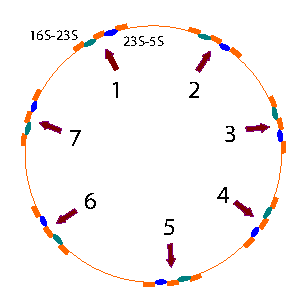
\includegraphics[width=80mm]{images/dna.pdf}
\caption[Pyroprinted regions of E. coli DNA]{Two sets of seven DNA sequences from unique copies of the 16S–23S (green) and 23S–5S (blue) ITS regions.}
\label{fig:dna}
\end{center}
\end{figure}

Dr. Black and Dr. Kitts of the Cal Poly Biology department have developed a library-dependent technique for comparing DNA fingerprints of bacterial isolates--specifically the identification and classification of E. coli strains. Pyroprinting refers to this library-dependent method of maintaining a database of pyroprints to represent genotypic information of bacterial isolates. Each pyroprint is generated from DNA of specific, highly variable regions in a microbial genome \cite{JanSoliman} call Intergenic Transcribed Spacers (ITS). Pyroprints are generated from two ITS regions around the rRNA genes in E. coli \cite{JanSoliman}. Between the 16S and 23S genes is the ITS region 16S-23S and between the 23S and 5S genes is the ITS region 23S-5S. There are typically seven copies of the rRNA operon in the E. coli genome and to generate a pyroprint all seven ITS loci are amplified and sequenced in a single reaction to maximix potential discrimination between strains \cite{JanSoliman}. There is variation between the 23S-5S region and the 16S-23S region in all seven loci of an E. coli sample. Pyrosequencing a single E. coli sample results in two pyroprints per isolate: one for the 16S-23S region and one for the 23S-5S region. A pyroprint is then represented as a vector of floating point values corresponding to the intensity of the reaction for each nucleotide released during the pyrosequencing reaction. Despite the relatively short sequence length from the pyrosequencers, the potential of discriminating between strains is maximized \cite{JanSoliman}. Pyroprints cannot be used to determine specific DNA sequences they are generated from, but rather they are a unique pattern analogous to a fingerprint of a microbe.

\subsection{CPLOP}
\label{cplop}

Pyroprinting is supported by a web-based database application that stores, retrieves, and analyzes isolates with their associated pyroprints as well as other relavant information, Cal Poly Library of Pyroprints (CPLOP) \cite{JanSoliman}. CPLOP is maintained by collecting samples from the environment, creating the pyroprints with pyrosequencing, managing a pyroprint library, then creating meaningful connections between samples. As the library grows to an appropriate size, unknown samples can then be compared with the database to determine their source. 

MST must include a method of determining similarity between microbes. In the case of CPLOP, there must be a way to compare similarity between pyroprints. CPLOP fulfills this requirement with a Pearson correlation between two pyroprint vectors of the same region \cite{AldrinMontana}.

In order to perform MST with our library of pyroprints, there must be a formally defined similarity between pyroprints. Cal Poly statistics student, Diana Shealy, conducted a study to determine pyroprint comparisons into three categories: definitely similar, definitely dissimilar, and reasonably similar \cite{DianaShealey}. She defined two values $\alpha$ and $\beta$ corresponding to the threshold for similarity and dissimilarity, respectively. A Pearson correlation score between $\alpha$ and $\beta$ might mean that a pair of pyroprints are similar, but it could also mean that a false negative or false positive has occured. Diana was able to determine thresholds where the number of false negatives are 1\%, 5\%, and 10\% at 0.9953, 0.9941, and 0.9915 respectively.

CPLOP \cite{JanSoliman} set the $\alpha$ and $\beta$ thresholds for CPLOP to be 0.995 and 0.99 respectively. These thresholds apply to both the 23S-5S and the 16S-23S regions.

If an isolate has several pyroprints for each ITS region, the similarity is based on a pairwise aggregation of the pyroprints for each region \cite{JanSoliman}.

\subsection{Strain Identification}
\label{strain-identification}

Pyroprints represent the genotype of each ITS region and this makes pyroprints an appropriate vehicle for determining similarity in genotypes between pairs of bacterial isolates. A strain a conglomeration of similar isolates where each isolate in the strain is of some similarity to all other isolates in the strain. The task of creating strains is then determining which isolates are similar which is representative of computationally determining clusters from our dataset. The definition of a strain can fit the definition of a cluster using the Pearson correlation as a similarity metric. The interpretation of each cluster is parallel to the concept of the bacterial strain, though there is no guarantee that each cluster correlates directly to a strain. Each cluster may represent a strain or at least closely resemble one.

\subsection{Agglomerative Heirarchical Clustering}

Partitional clustering algorithms like K-means clustering work by developing centroids and then assigning data points based on the distance from centroids \cite{Liu}. Partitional algorithms work best when there is an estimate number of clusters, but there is no estimate of number of strains when clustering begins. As new data is added to the database it becomes more difficult to estimate the number of clusters and K-means becomes less reliable. A clustering algorithm based on agglomerative hierarchical clustering is utilized by CPLOP due to no apriori knowledge of the number of partitions \cite{JanSoliman}. In hierarchical clustering, each item starts in it’s own cluster. Items are groups by a similarity to other clusters by combining two clusters. The two clusters with the highest similarity are grouped first, then the next more similar clusters, and soon until the items are in a single cluster. The result is a dendrogram. Items clustered earlier are more similar and items clustered later are less similar, and there is still some similarity score that connects each cluster. Hierarchical clustering solves the problem of an unknown number of clusters by allowing any threshold of similarity and the resulting clusters.
